\begin{samplecase}
{\bf Fission yields and neutron observables n + ${}^{239}$Pu}\newline
Since 2020, TALYS has the option to start a calculation with a pre-defined fission fragment (FF) distribution and to explicitly 
calculate the neutron and gamma decay from that, leading to fission product yields (FPY) and various fission neutron observables. 
In these sample cases for thermal neutrons on ${}^{239}$Pu, 3 different FF models are compared with regards to the resulting 
FPY and neutron distributions. The prompt neutron multiplicity as a function of mass, 
$\overline{\nu}(A)$, number of neutrons, $P({\nu})$, the total average,
$\overline{\nu}$, and the prompt fission neutron spectrum,
are calculated, as well as the fission product yields as a 
function of $Z$ and $A$.
The following input file for the GEF model is used

\VerbatimInput{\samples n-Pu239-fy-gef/org/talys.inp}

and similarly for the HF3D model ({\bf ffmodel 2}) and SPY model ({\bf ffmodel 3}).
The FY calculation can be somewhat time consuming so the sample cases are done only for thermal neutron energy. Not however that the usual incident energy file can also be used to obtain e.g. $\overline{\nu}$ as a function of incident energy.
In Fig. \ref{n-Pu239-FY} the FPY results for the 3 models are plotted together with the FPY from ENDF/B-VIII.0. These FPY as a function of A are given in file {\it yieldA1.00E-06.fis}.
Fig. \ref{n-Pu239-FY-nuA} presents the distribution of $\overline{\nu}(A)$ as a function of fission product mass. This is given in output 
file {\it nunA1.00E-06.fis}.
Fig. \ref{n-Pu239-FY-Pnu} presents the distribution of $\nu$ as a function of number of neutrons, for an incident energy of 1 MeV. This is given in output 
file {\it Pnun1.00E-06.fis}.
The prompt fission neutron spectrum of Fig. \ref{n-Pu239-FY-PFNS} is given in file {\it pfns1.00E-06.fis}.
In the addition to the latter case, in {\it n-Pu239-fy-pfns} we have also done a TALYS run without explicit FY evaporation, 
which means the phenomenologicla model of Iwamoto model for PFNS is automatically used.
\end{samplecase}
\begin{figure}
\centering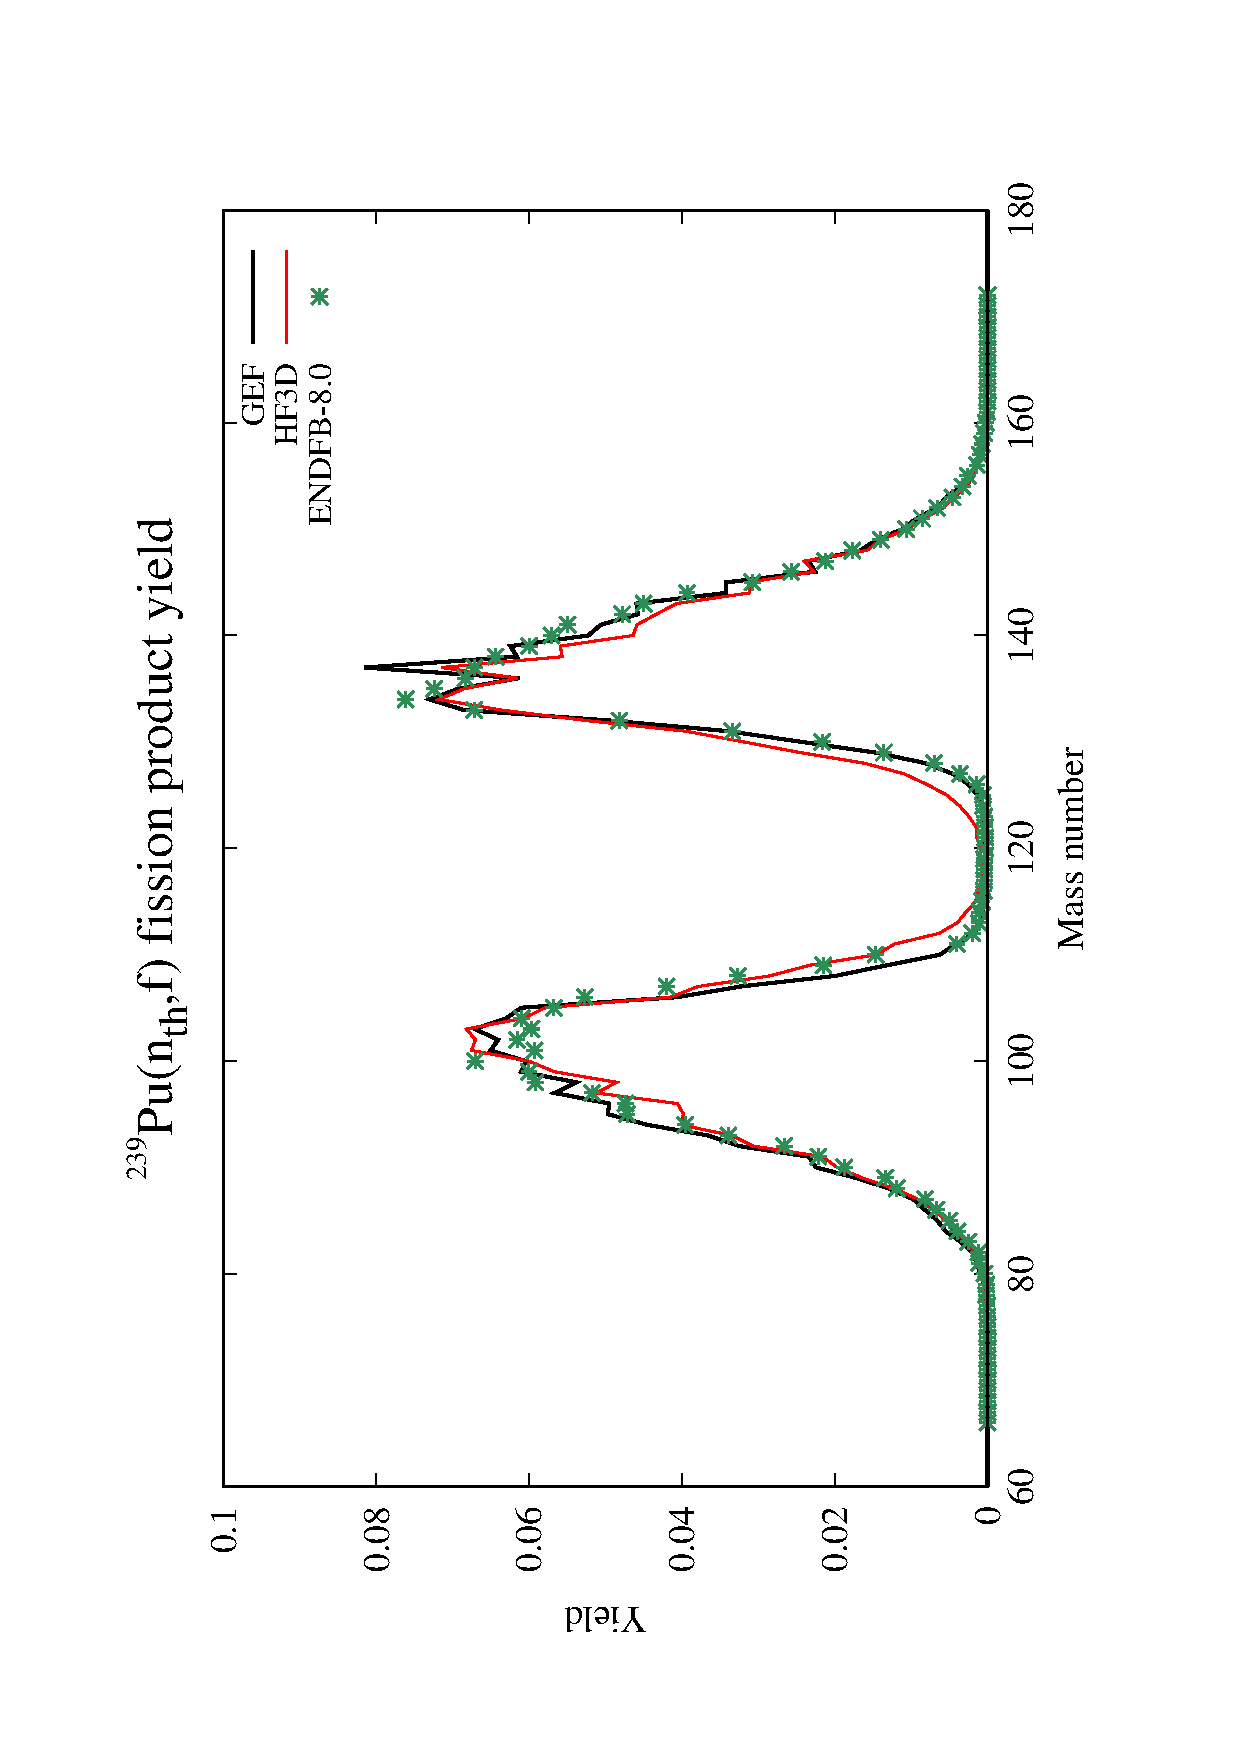
\includegraphics[scale=0.5,angle=270]{n-Pu239-FY}
\caption{Fission product yields for  n$_{th}$ + $^{239}$Pu, for 3 FF models.}
\label{n-Pu239-FY}
\end{figure}
\begin{figure}
\centering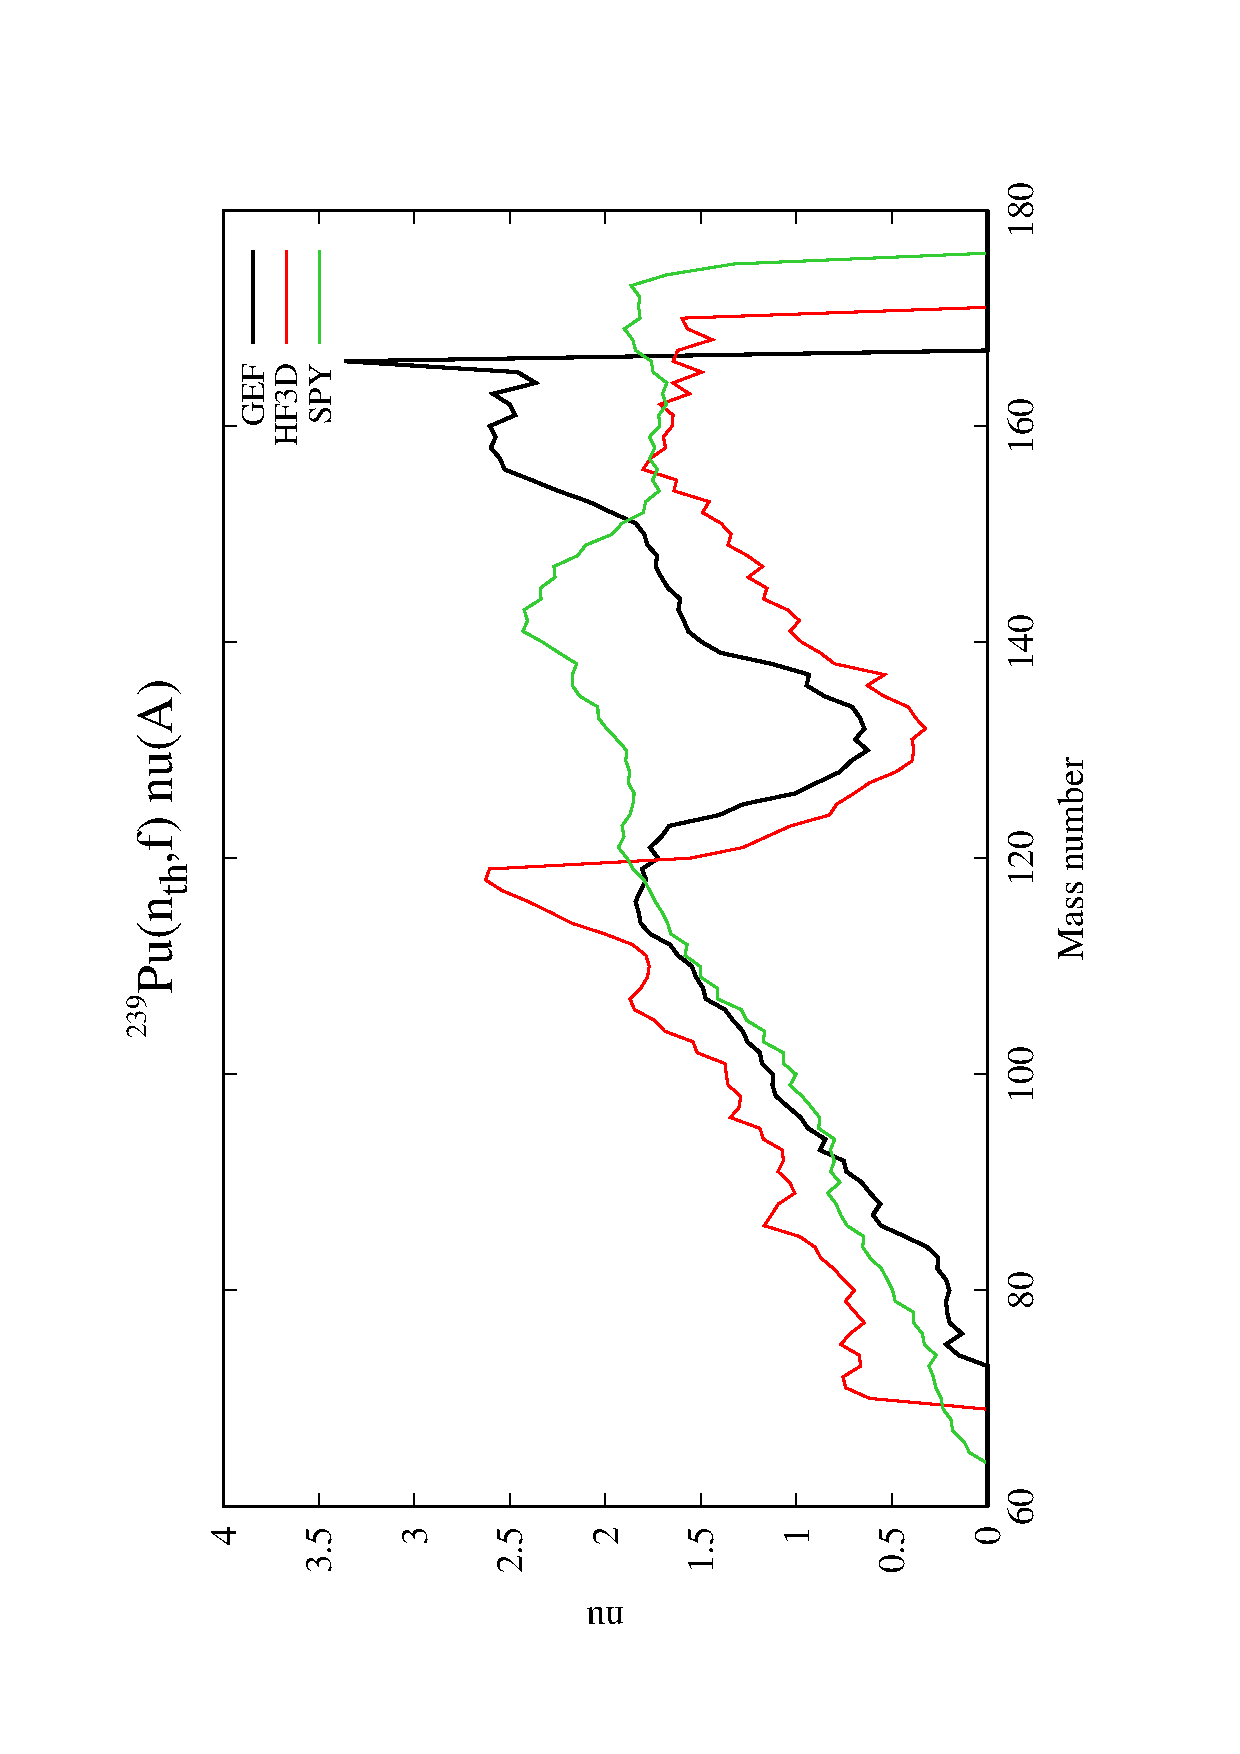
\includegraphics[scale=0.5,angle=270]{n-Pu239-FY-nuA}
\caption{Prompt neutron multiplicity $\overline{\nu}(A)$, as a function of fission product mass, for n$_{th}$ + $^{239}$Pu, for 3 FF models.}
\label{n-Pu239-FY-nuA}
\end{figure}
\begin{figure}
\centering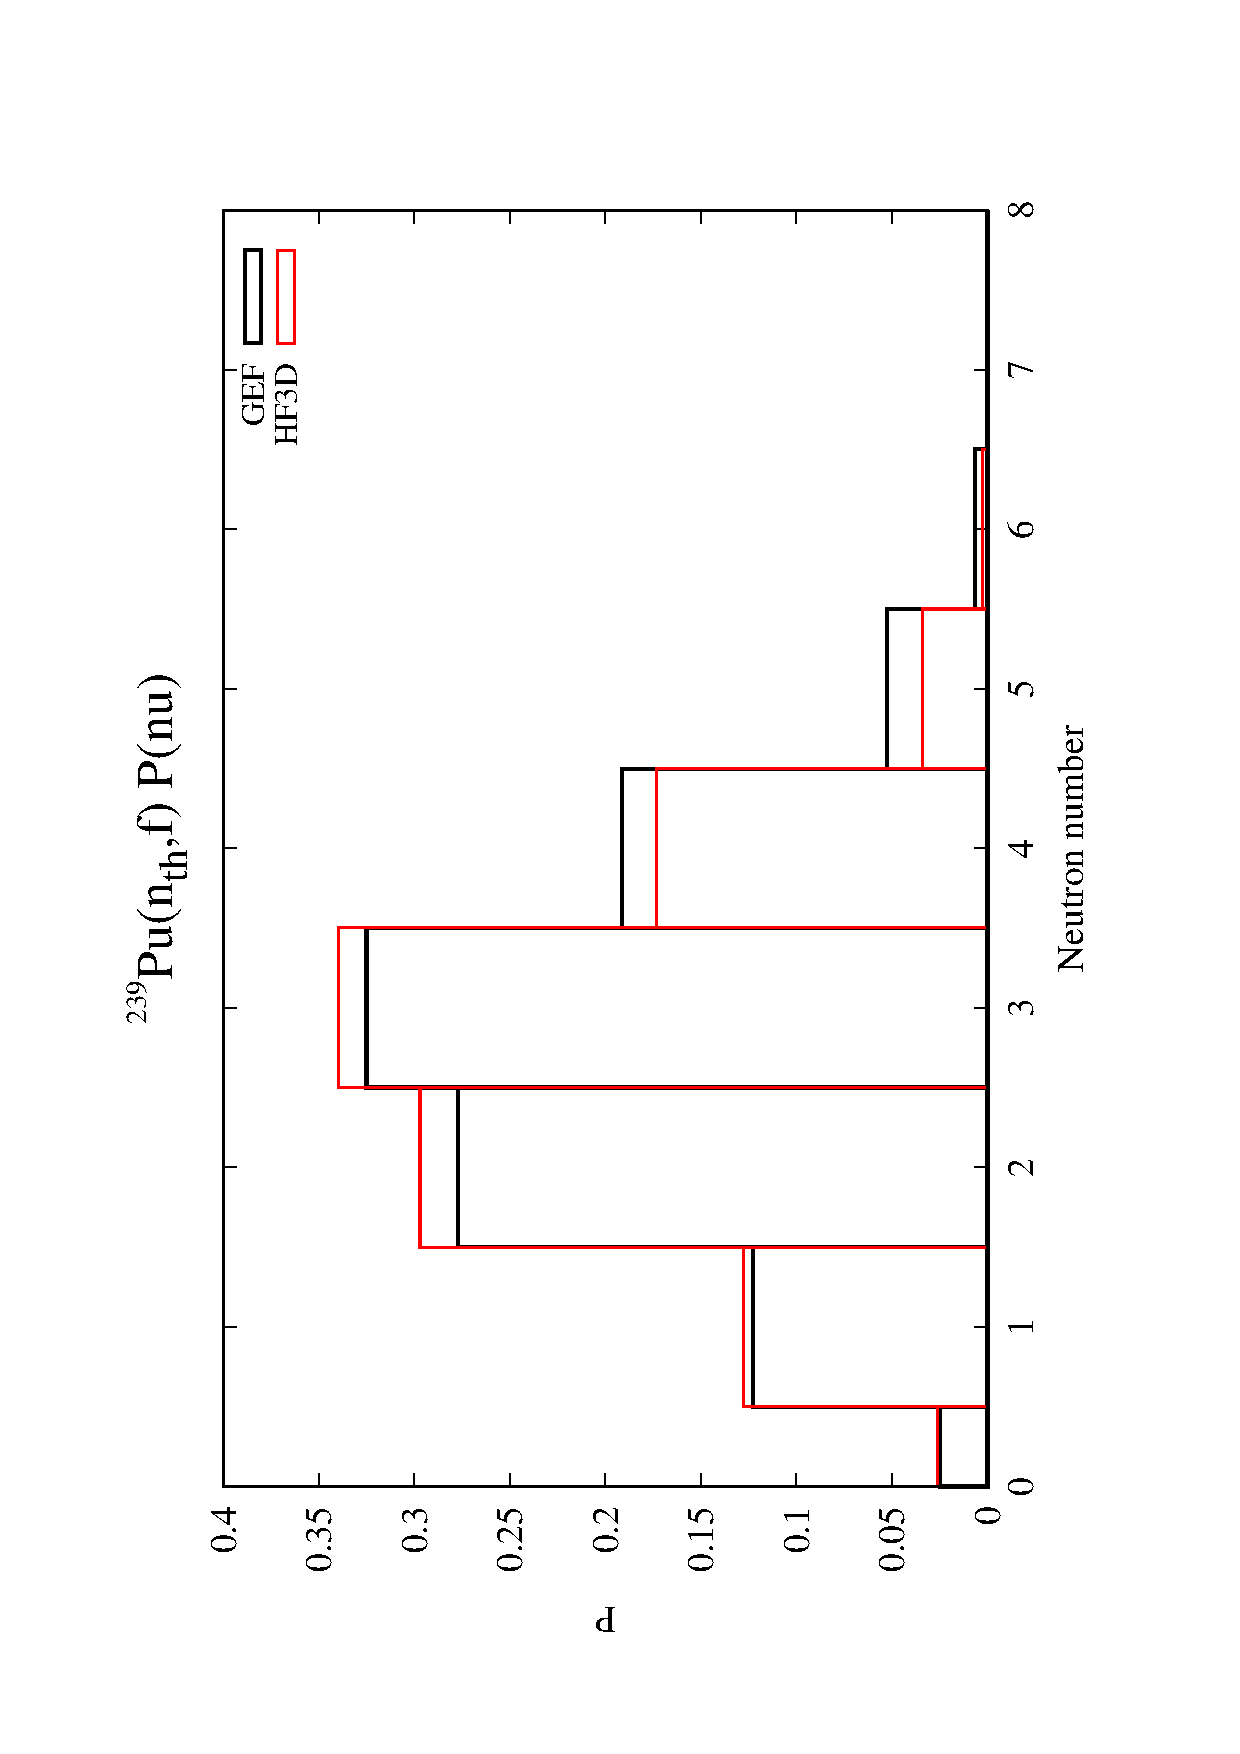
\includegraphics[scale=0.5,angle=270]{n-Pu239-FY-Pnu}
\caption{Prompt neutron multiplicity distribution $P(\nu )$, for n$_{th}$ + $^{239}$Pu, for 3 FF models.}
\label{n-Pu239-FY-Pnu}
\end{figure}
\begin{figure}
\centering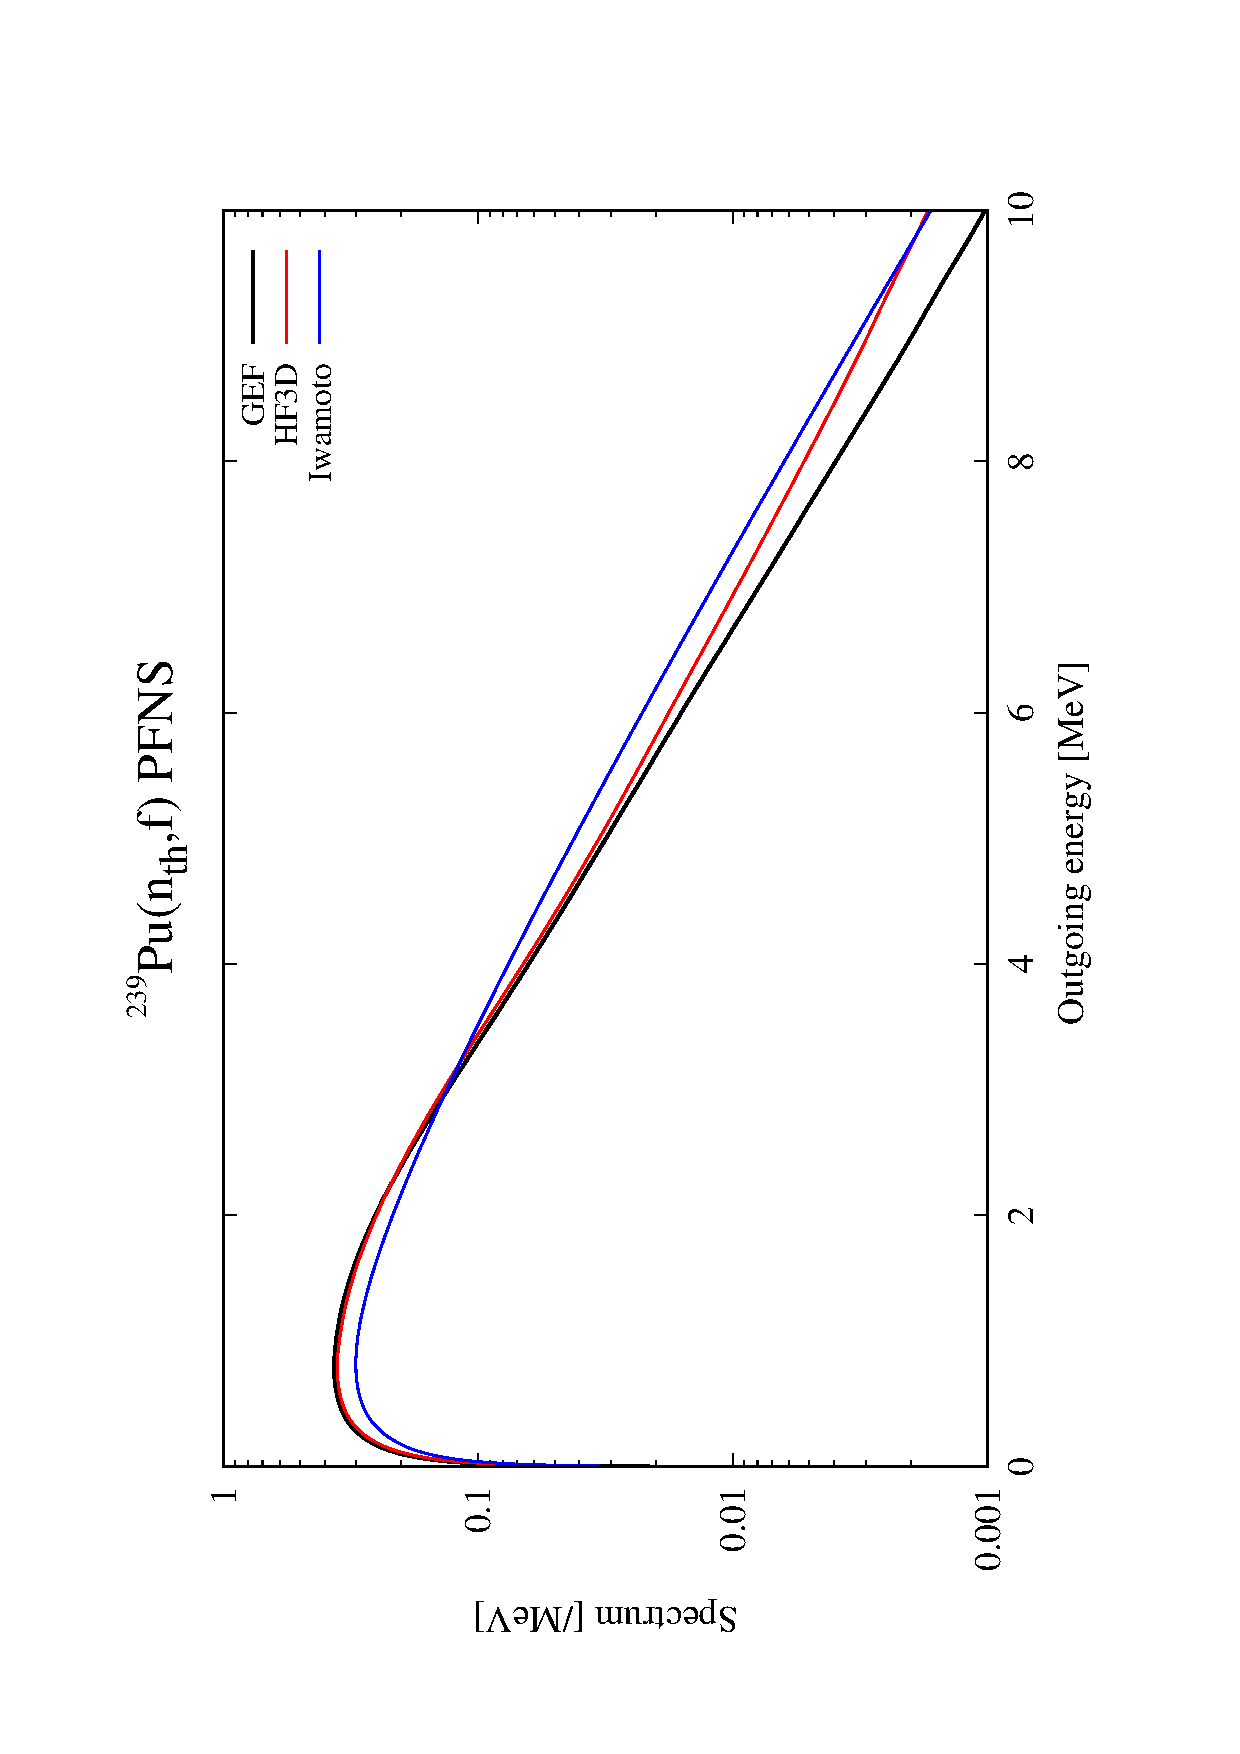
\includegraphics[scale=0.5,angle=270]{n-Pu239-FY-PFNS}
\caption{Prompt fission neutron spectrum, for n$_{th}$ + $^{239}$Pu, for 3 FF models.}
\label{n-Pu239-FY-PFNS}
\end{figure}
